\documentclass[tikz,border=5pt]{standalone}
\usepackage[UTF8]{ctex}\usepackage{amsmath,amssymb}
\usetikzlibrary{arrows.meta,calc}
\definecolor{ink}{HTML}{243447}\definecolor{blue}{HTML}{2765A2}
\definecolor{green}{HTML}{3F7D5B}\definecolor{red}{HTML}{B74739}
\tikzset{body/.style={draw=ink,thick},vec/.style={draw=blue,thick,-{Latex}},guide/.style={gray!65,dashed},dim/.style={ink,{Latex}-{Latex}},line cap=round,line join=round}
\begin{document}
\begin{tikzpicture}[x={(1cm,0cm)},y={(.45cm,.32cm)},z={(0cm,1cm)}]
 \fill[blue!4](0,0,0)--(6,0,0)--(6,2,0)--(0,2,0)--cycle;
 \draw[body](0,0,0)--(6,0,0)--(6,.7,0);
 \draw[body](0,2,0)--(6,2,0)--(6,1.3,0);
 \draw[body,fill=gray!20](5.83,.7,0)--(6.17,.7,0)--(6.17,1.3,0)--(5.83,1.3,0)--cycle;
 \node[right]at(6.2,1,0){$R$};
 \draw[ink,line width=2pt](1,-.25,0)--(1,2.25,0)node[above]{$m$};
 \draw[vec](1.2,.3,0)--(2.7,.3,0)node[midway,below]{$v_0$};
 \draw[guide,-{Latex}](1.2,1.6,0)--(2.7,1.6,0)node[midway,above]{$F_x$正向};
 \draw[vec](4,1,0)--(4,1,1.65)node[above]{$\boldsymbol B$};
 \draw[dim](-.4,0,0)--(-.4,2,0)node[midway,left]{$l$};
 \draw[vec](5,-1,0)--(6.2,-1,0)node[right]{$x$};
 \node at(3,-2,0){导轨平面水平；$z$方向竖直向上};
\end{tikzpicture}
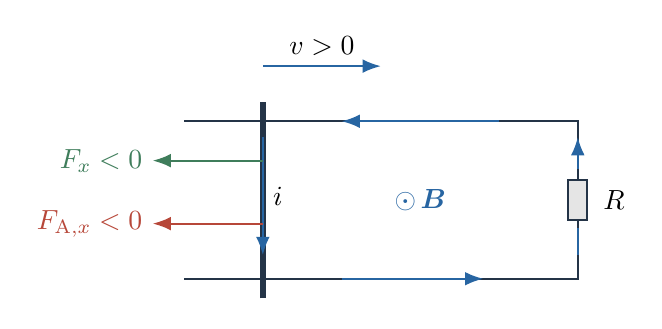
\begin{tikzpicture}
 \draw[body](0,0)--(5,0)--(5,.75)(0,2)--(5,2)--(5,1.25);
 \draw[body,fill=gray!20](4.88,.75)rectangle(5.12,1.25);
 \draw[ink,line width=2pt](1,-.25)--(1,2.25);
 \draw[vec](1,1.8)--(1,.3)node[midway,right]{$i$};
 \draw[vec](2,.0)--(3.8,.0);
 \draw[vec](4,2)--(2,2);
 \draw[vec](5,.3)--(5,.65)(5,1.4)--(5,1.8);
 \node[blue]at(3,1){$\odot\,\boldsymbol B$};
 \draw[red,thick,-{Latex}](1,.7)--(-.4,.7)node[left]{$F_{\mathrm A,x}<0$};
 \draw[green,thick,-{Latex}](1,1.5)--(-.4,1.5)node[left]{$F_x<0$};
 \draw[vec](1,2.7)--(2.5,2.7)node[midway,above]{$v>0$};
 \node[right]at(5.2,1){$R$};
\end{tikzpicture}
\begin{tikzpicture}[x=4.5cm,y=2.7cm]
 \draw[vec](0,0)--(1.15,0)node[right]{$x/x_{\mathrm s}$};
 \draw[vec](0,0)--(0,1.2)node[above]{$i/i_0$};
 \draw[blue,thick,domain=0:1,samples=101]plot(\x,{sqrt(1-\x)});
 \draw[guide](.75,0)--(.75,.5)--(0,.5);
 \node[left]at(0,.5){$1/2$};\node[left]at(0,1){$1$};
 \node[below]at(.75,0){$3/4$};\node[below]at(1,0){$1$};
 \fill[green](.75,.5)circle(.015);\fill[green](1,0)circle(.015);
\end{tikzpicture}
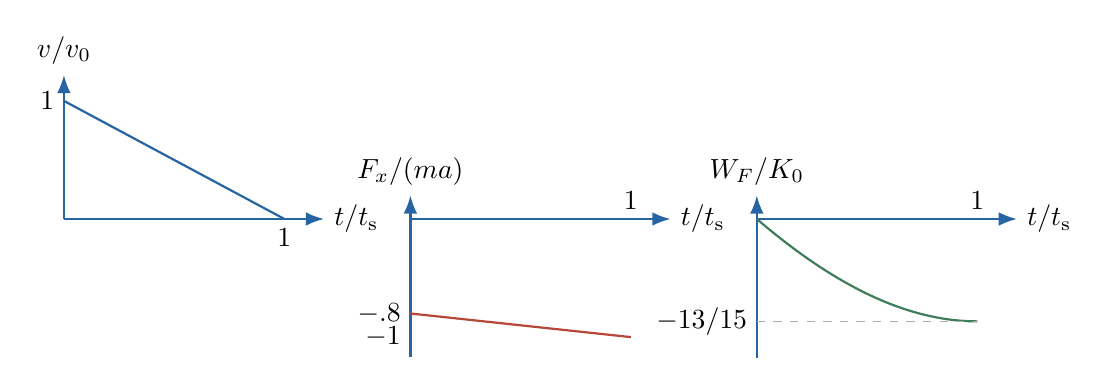
\begin{tikzpicture}
 \begin{scope}[x=2.8cm,y=1.5cm]
 \draw[vec](0,0)--(1.18,0)node[right]{$t/t_{\mathrm s}$};
 \draw[vec](0,0)--(0,1.22)node[above]{$v/v_0$};
 \draw[blue,thick](0,1)--(1,0);\node[left]at(0,1){$1$};\node[below]at(1,0){$1$};
 \end{scope}
 \begin{scope}[shift={(4.4,0)},x=2.8cm,y=1.5cm]
 \draw[vec](0,0)--(1.18,0)node[right]{$t/t_{\mathrm s}$};
 \draw[vec](0,-1.17)--(0,.2)node[above]{$F_x/(ma)$};
 \draw[red,thick](0,-.8)--(1,-1);
 \node[left]at(0,-.8){$-.8$};\node[left]at(0,-1){$-1$};
 \node[above]at(1,0){$1$};
 \end{scope}
 \begin{scope}[shift={(8.8,0)},x=2.8cm,y=1.5cm]
 \draw[vec](0,0)--(1.18,0)node[right]{$t/t_{\mathrm s}$};
 \draw[vec](0,-1.18)--(0,.2)node[above]{$W_F/K_0$};
 \draw[green,thick,domain=0:1,samples=81]plot(\x,{-1.6*\x+.6*\x*\x+(2/15)*\x*\x*\x});
 \node[left]at(0,-.8667){$-13/15$};\node[above]at(1,0){$1$};
 \draw[guide](0,-.8667)--(1,-.8667);
 \end{scope}
\end{tikzpicture}
\end{document}
